\section{Solar System Orbits}

\lstinputlisting[caption={Code to collect the positions and velocities of solar system objects and apply the LeapFrog and Runge-Kutta 4 Algorithms.}]{orbits.py}

In this section we will simulate the orbits of the planets in our Solar system. Here the forces between planets are negligible compared to the force between each planet and the sun. The orbit of each planet is therefore well defined by a single equation, which we can easily brute force with an ODE solver. The acceleration of the planet is given by the gravitational force, which is defined as

\begin{equation}
    \vec{F_G} = \frac{-mMG}{||\vec{r}||^3} \vec{r}.
\end{equation}

Where $M = 1.989 \times 10^{30}$ kg is the mass of the sun, $m$ is the mass of the planet, $G = 6.6743 \times 10^{-11}$ m$^3$ kg$^{-1}$ s$^{-2}$ is the gravitational constant. $\vec{r}$ is the vector pointing from is the planet to the sun. The acceleration is then simply given through $F = ma$, so the planet mass cancels out.

We get the initial positions and velocities of all 8 solar system planets and the sun using \texttt{astropy} following the procedure given on the handin at 10:00 on 2021-12-07. We show these initial positions in Figure \ref{fig:initial_pos}.

\begin{figure}
    \centering
    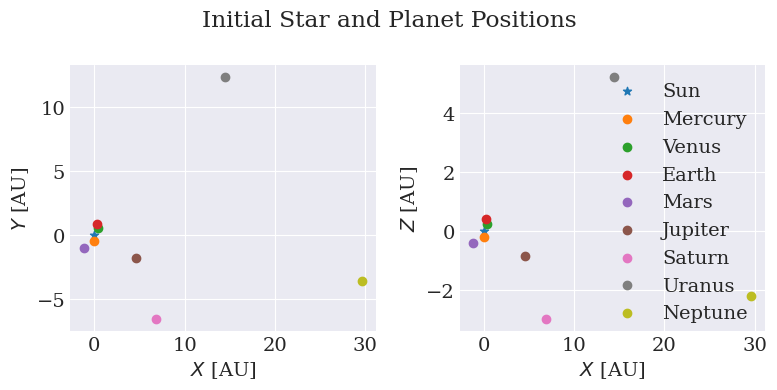
\includegraphics[width=\textwidth]{results/initial_positions.png}
    \caption{Initial positions of all 8 solar system planets and the sun at 10:00 on 2021-12-07 in the x-y plane (\textit{left}) and the x-z plane (\textit{right})}. 
    \label{fig:initial_pos}
\end{figure}


\subsection{Leapfrog}

\lstinputlisting[caption={LeapFrog Class}, linerange={5-64}]{algorithms.py}

We start by applying the leapfrog algorithm to simulate the orbits. This is the proper method of solving ordinary differential equations for phsyical systems, because it is reversible and therefore able to conserve energy. This is an important factor in making sure the solutions do not diverge to unphysical states. We have implemented the algorithm in a class, given above. The leapfrog algorithm works by kicking the object from positions $x_i$ with velocity $v_{i+1/2}$. However, we are only given $x_0$ and $v_0$. This means that we first have to use a regular ODE solver to find $v_{1/2}$. Here, this is done in the \texttt{\_kickstart} function with a single iteration of Runge-Kutta 4.

We integrate the orbits with a step size $h = 0.5$ days for 200 years, this gives $N = 146100$ steps in total. We show the resulting orbits in Figure \ref{fig:orbits_lf}.

\begin{figure}
    \centering
    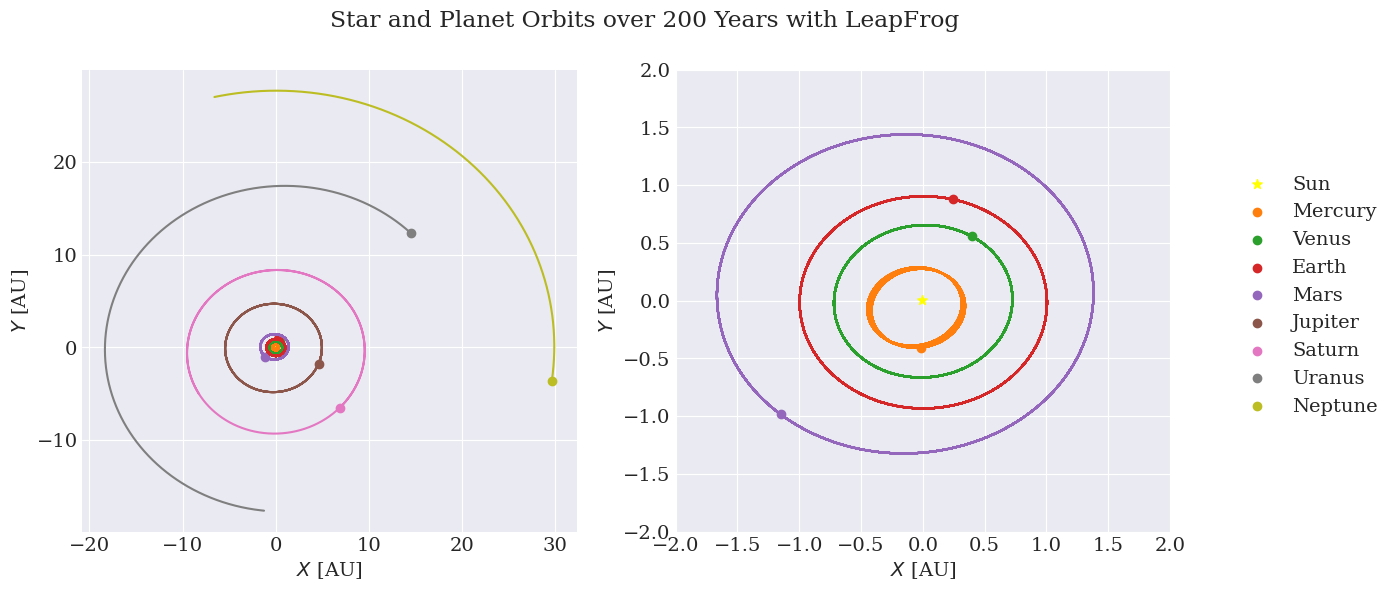
\includegraphics[width=\textwidth]{results/orbits_lf.png}
    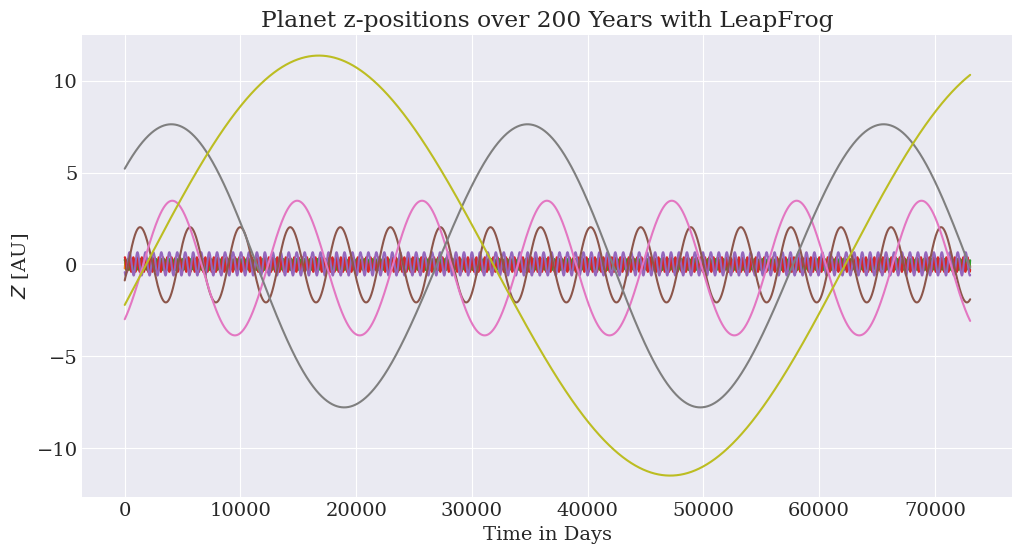
\includegraphics[width=0.6\textwidth]{results/zplane.png}
    \caption{Integrated orbits of the 8 planets in the solar system over 200 years with a step size of 0.5 days using the LeapFrog algorithm and an initial kick with Runge-Kutta 4. \textit{top}: Planetary orbits in the x-y plane, the plot in the right is zoomed in to better highlight the orbits of the rocky planets. \textit{bottom}: Planetary positions on the z-axis as a function of time.}
    \label{fig:orbits_lf}
\end{figure}

The orbits appear to behave very nicely. As mentioned previously, this algorithm conserves energy. This is visible in the fact that the orbits in the top plot of Figure \ref{fig:orbits_lf} appear to be well defined lines that do not diverge away from or towards the Sun, which would be a violation of energy conservation. This same fact is visible in the bottom plot, the planets all appear to oscilate up and down in the z-plane, but the amplitude of the oscilations is constant. This also indicates the fact that energy conservation is not violated. Finally, this simulation shows that the orbit of Mercury is not entirely constant, but rather shifts around a little bit. This is not per se an inconsistent result, because its orbit remains closed.

\subsection{Runge-Kutta 4}

\lstinputlisting[caption={Runge-Kutta 4 Class}, linerange={67-118}]{algorithms.py}

As an experiment, we also integrate the orbits of the planets given the same initial conditions with a normal ODE solver that does not have the power to preserve energy. Similar to the LeapFrog method above, we also implement the RK-4 method using a class given above. However, this time we do not have to provide the velocities with an initial kick. We use the same step size and number of steps as before, and plot the resulting orbits in Figure \ref{fig:orbits_rk4}

\begin{figure}
    \centering
    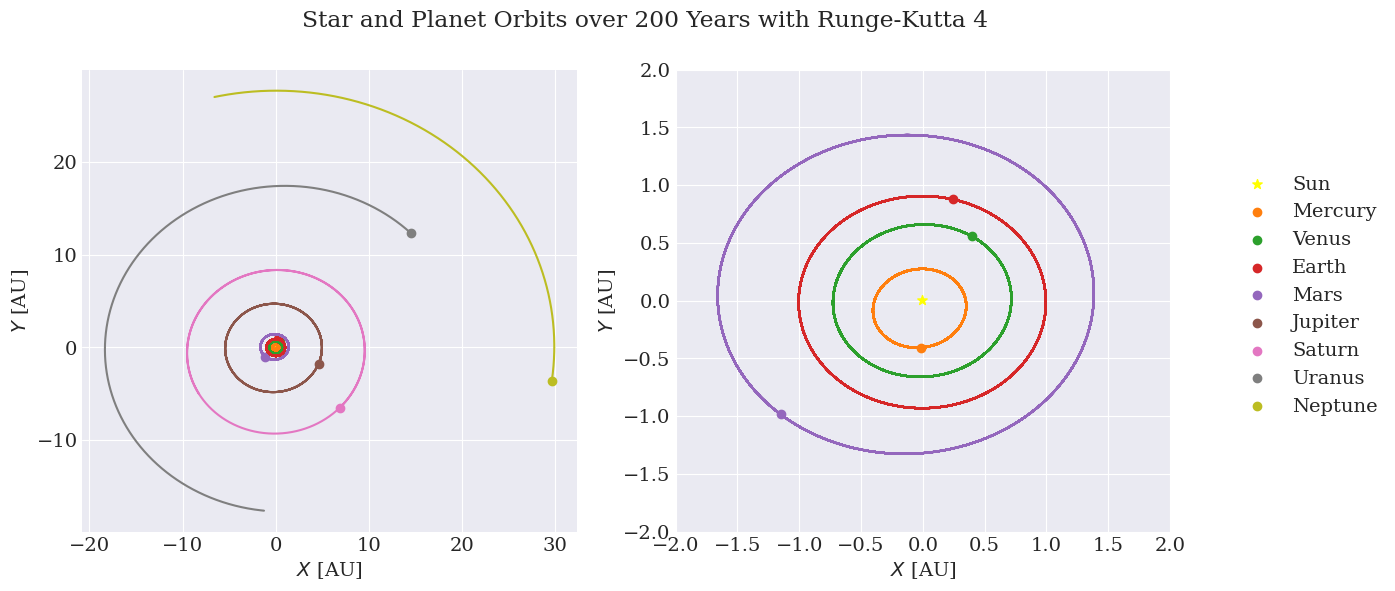
\includegraphics[width=\textwidth]{results/orbits_rk4.png}
    \caption{Integrated orbits in the x-y plane of the 8 planets in the solar system over 200 years with a step size of 0.5 days using the Runge-Kutta 4 method.}
    \label{fig:orbits_rk4}
\end{figure}

Visually, the orbits of all planets except Mercury appear exactly the same. The biggest difference lies in the fact that Mercury's orbit remains constant over 200 years according to RK4, while it shifted around according to LeapFrog. However comparing two plots with each other visually is not the best method of investigating the performance of an algorithm. Therefore we present the difference in x-position between the two integrated orbits in Figure \ref{fig:orbits_diff}. 

In that figure we see that the difference in x-position shows a somewhat periodic pattern that increases in amplitude over time. This indicates that the two solutions are slowly diverging from each other. The pattern we see corresponds to what we might have expected. Because RK-4 is a forward method, the velocity it predicts will always push the object slightly more away from the star than the true value. This small error accumulates over time leading to a larger orbit. This can physically be interpreted as increasing the amount of energy in the system, which is a violation of the laws of physics that LeapFrog was able to adhere to. Additionaly, we can clearly see that there is a large discrepancy between the two orbits of Mercury that occurs from a very early point.

\begin{figure}
    \centering
    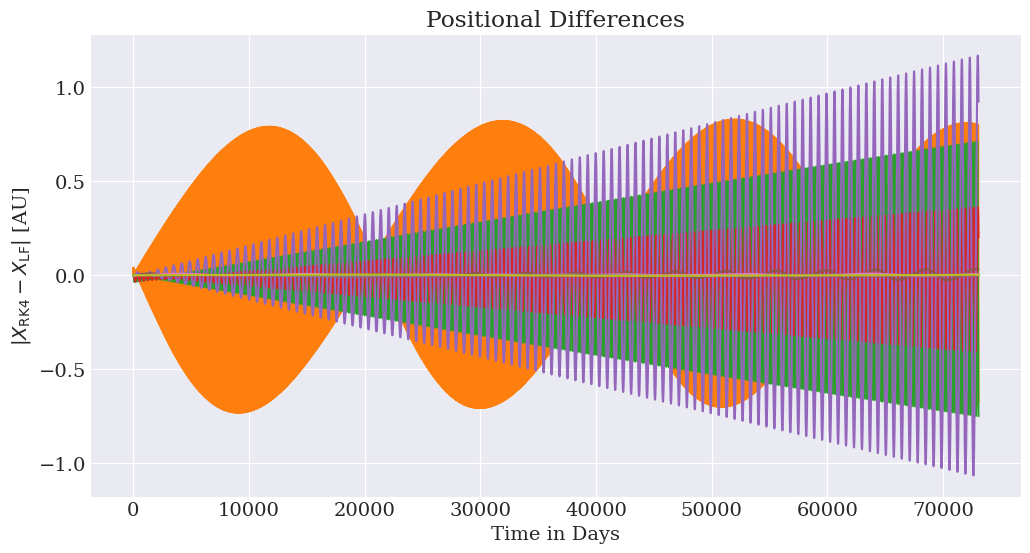
\includegraphics[width=0.6\textwidth]{results/rk4_lf_diff.png}
    \caption{Difference in x-position between the orbit as integrated using the Runge-Kutta 4 method and the LeapFrog algorithm plotted as a function of time}
    \label{fig:orbits_diff}
\end{figure}









